\documentclass[12pt]{article}
\usepackage[utf8]{inputenc}
\usepackage{amsfonts}
\usepackage{graphicx}
\usepackage{amsmath}
\usepackage{geometry}
\usepackage{hyperref}
\usepackage{chngcntr}
\counterwithin{figure}{section}
\geometry{a4paper, margin=1in}
\newcommand{\VAR}[1]{\mathbf{#1}}
\newcommand{\T}{\mathbb{T}}
\title{Energy Flow Optimization Report}
\author{Amine Abdellaziz}
\date{\today}

% Do we put figures generated by Pyomo or AMPL?
%\graphicspath{{figs/}{figs/pyomo/}}
\graphicspath{{figs/}{figs/ampl/}}

\begin{document}

\maketitle

\begin{abstract}
This report details the optimization of energy flows within a system comprising a photovoltaic (PV) system, an electrical battery, a connection to the external electrical grid, and a consumer. The primary objective is to meet the predicted electrical energy demands while minimizing costs.
\end{abstract}

\section{Problem Description}
The problem description can be found in the instructions of the \href{https://github.com/mathaziz/energy_flow_optimization/blob/main/instructions_hymate.pdf}{hymate document}.

\subsection{Parameters}
\begin{figure}[h]
    \centering
    \includegraphics[width=\textwidth]{input_data}
    \caption{The data of the problem.}
    \label{fig:data}
\end{figure}

The parameters of the problem are as follows, with given values illustrated in Figure \ref{fig:data}:
\begin{itemize}
    \item \(pv_t\): Predicted photovoltaic production at time \(t\) (kW).
    \item \(conso_t\): Predicted consumption at time \(t\) (kW).
    \item \(lcos_t\): Levelized cost of storage at time \(t\) (cents/kWh), where \(lcos_t = 9.3\) is constant.
    \item \(sell_t\): Selling price of the energy at time \(t\) (cents/kWh).
    \item \(buy_t\): Buying price of the energy at time \(t\) (cents/kWh).
\end{itemize}

\subsection{Solving Methodology}
The problems have been modeled and solved in Python using \href{https://dev.ampl.com/ampl/python/index.html}{AMPL}.

\section{Part A}

\subsection{Variables}
\begin{figure}[h]
    \centering
    \includegraphics[width=\textwidth]{diagram}
    \caption{The different flows representing the variables.}
    \label{fig:diagram}
\end{figure}

The variables of the model for Part A are illustrated in Figure \ref{fig:diagram} and are defined as follows:
\begin{itemize}
    \item \(\VAR{pvg_t}\): Flow from the photovoltaic system to the grid at time \(t\) (kW).
    \item \(\VAR{pvc_t}\): Flow from the photovoltaic system to the consumer at time \(t\) (kW).
    \item \(\VAR{pvb_t}\): Flow from the photovoltaic system to the battery at time \(t\) (kW).
    \item \(\VAR{gb_t}\): Flow from the grid to the battery at time \(t\) (kW).
    \item \(\VAR{gc_t}\): Flow from the grid to the consumer at time \(t\) (kW).
    \item \(\VAR{bg_t}\): Flow from the battery to the grid at time \(t\) (kW).
    \item \(\VAR{bc_t}\): Flow from the battery to the consumer at time \(t\) (kW).
    \item \(\VAR{charge_t}\): Charge level of the battery at time \(t\) (kWh).
\end{itemize}

All variables are non-negative real values, and the set of all time steps/indices is represented by the set \(\T \subset \mathbb{N}\).

\subsection{Objective Function}
The objective function describing the cost is:

\begin{equation}
    \min \text{Cost} = \sum_{t \in \T} \left( buy_t \cdot eb_t - sell_t \cdot es_t + lcos_t \cdot ed_t \right),
    \label{eq:cost}
\end{equation}

where at each time step \(t \in \T\):
\begin{itemize}
    \item The bought energy \(eb_t = \VAR{gb_t} + \VAR{gc_t}\) is the sum of the grid to battery flow (\(\VAR{gb_t}\)) and the grid to consumer flow (\(\VAR{gc_t}\)).
    \item The sold energy \(es_t = \VAR{bg_t} + \VAR{pvg_t}\) is the sum of the battery to grid flow (\(\VAR{bg_t}\)) and the photovoltaic system to grid flow (\(\VAR{pvg_t}\)).
    \item The discharged energy \(ed_t = \VAR{bc_t} + \VAR{bg_t}\) is the sum of the battery to consumer flow (\(\VAR{bc_t}\)) and the battery to grid flow (\(\VAR{bg_t}\)).
\end{itemize}

\subsection{Constraints}
The constraints of the problem are described as follows:

\textbf{Photovoltaic Production:}
\begin{equation}
    \VAR{pvg_t} + \VAR{pvc_t} + \VAR{pvb_t} \leq pv_t, \quad \forall t \in \T
\end{equation}

\textbf{Battery:}
We ensure that the charge level of the battery does not exceed its capacity:
\begin{equation}
    \VAR{charge_t} \leq 160, \quad \forall t \in \T.
    \label{eq:charge}
\end{equation}

We also ensure that the maximum charge and discharge capabilities are respected:
\begin{align}
\text{(Max discharge)} & \quad \VAR{bg_t} + \VAR{bc_t} \leq 100, \quad \forall t \in \T \\
\text{(Max charge)} & \quad \VAR{gb_t} + \VAR{pvb_t} \leq 100, \quad \forall t \in \T
\end{align}

Evolution of the level of charge in the battery:
\begin{equation}
    \VAR{charge_t} =
    \begin{cases}
        0.92 \cdot (\VAR{gb_t} + \VAR{pvb_t}) - (\VAR{bg_t} + \VAR{bc_t}) & \text{if } t = 0 \\
        \VAR{charge_{t-1}} + 0.92 \cdot (\VAR{gb_t} + \VAR{pvb_t}) - (\VAR{bg_t} + \VAR{bc_t}) & \text{for } t \neq 0
    \end{cases}
\end{equation}

\textbf{Grid:}
\begin{align}
\text{(Max sell power)} & \quad \VAR{bg_t} + \VAR{pvg_t} \leq 700, \quad \forall t \in \T \\
\text{(Max buy power)} & \quad \VAR{gb_t} + \VAR{gc_t} \leq 700, \quad \forall t \in \T
\end{align}

\textbf{Consumer Demands:}
\begin{equation}
    \VAR{gc_t} + \VAR{pvc_t} + \VAR{bc_t} = conso_t, \quad \forall t \in \T
\end{equation}

\subsection{Results}
\begin{figure}[p]
    \centering
    \includegraphics[width=\textwidth]{PartA/pv_output}
    \caption{Distribution of the photovoltaic output.}
\end{figure}

\begin{figure}[p]
    \centering
    \includegraphics[width=\textwidth]{PartA/grid}
    \caption{Energy contribution to and from the grid.}
\end{figure}

\begin{figure}[p]
    \centering
    \includegraphics[width=\textwidth]{PartA/battery}
    \caption{Charge level and contribution of the battery.}
    \label{fig:batteryA}
\end{figure}

\begin{figure}[p]
    \centering
    \includegraphics[width=\textwidth]{PartA/consumer_input}
    \caption{Energy mix to the consumer.}
    \label{fig:solA}
\end{figure}

\pagebreak

\section{Part B}

\subsection{Modelling Constraints for Grid Transactions}
Assume the same model as Part A. To prevent simultaneous buying and selling from the grid, we introduce two binary variables:
\begin{itemize}
    \item \(\mathbf{to\_buy}_t \in \{0, 1\}\): Indicates whether we are buying energy from the grid (\(1\)) or not (\(0\)) at time \(t\).
    \item \(\mathbf{to\_sell}_t \in \{0, 1\}\): Indicates whether we are selling energy to the grid (\(1\)) or not (\(0\)) at time \(t\).
\end{itemize}

We add a constraint to ensure that buying and selling do not occur at the same time:
\begin{equation}
    \mathbf{to\_buy}_t + \mathbf{to\_sell}_t \leq 1, \quad \forall t
\end{equation}

Additionally, we introduce two constraints (through the Big-M method) to enforce the effect of the binary variables on the energy flows:
\begin{align}
    \mathbf{gb}_t + \mathbf{gc}_t \leq \mathbf{to\_buy}_t \cdot M, \quad \forall t \\
    \mathbf{bg}_t + \mathbf{pvg}_t \leq \mathbf{to\_sell}_t \cdot M, \quad \forall t
\end{align}

where \(M > 0\) is any sufficiently large number (we took \(M = 10^5\)).

\subsection{Results}
\begin{figure}[p]
    \centering
    \includegraphics[width=\textwidth]{PartB/pv_output}
    \caption{Distribution of the photovoltaic output.}
\end{figure}

\begin{figure}[p]
    \centering
    \includegraphics[width=\textwidth]{PartB/grid}
    \caption{Energy contribution to and from the grid.}
\end{figure}

\begin{figure}[p]
    \centering
    \includegraphics[width=\textwidth]{PartB/battery}
    \caption{Charge level and contribution of the battery. Compare with Figure \ref{fig:batteryA} and notice how we do not simultaneously buy and sell.}
    \label{fig:batteryB}
\end{figure}

\begin{figure}[p]
    \centering
    \includegraphics[width=\textwidth]{PartB/consumer_input}
    \caption{Energy mix to the consumer. By adding constraints on how we buy and sell energy, we increase the optimal cost compared to the solution in Figure \ref{fig:solA}.}
\end{figure}

\pagebreak

\section{Part C}

\subsection{Modelling}

\subsubsection{Sell and Buy in Packages}
We assume the same model as in Part B. To model the fact that we are allowed to only buy and sell in \(100\) kWh packages, we introduce four new integer variables:
\begin{itemize}
    \item \(\VAR{pvgn_t}\): Number of packages (\(\in \mathbb{N}\)) sold from the PV to the grid.
    \item \(\VAR{gbn_t}\): Number of packages (\(\in \mathbb{N}\)) bought from the Grid to the Battery.
    \item \(\VAR{gcn_t}\): Number of packages (\(\in \mathbb{N}\)) bought from the Grid to the Consumer.
    \item \(\VAR{bgn_t}\): Number of packages (\(\in \mathbb{N}\)) sold from the Battery to the Grid.
\end{itemize}

We then redefine the following variables:
\begin{align}
    \VAR{pvg_t} &= 100 \times \VAR{pvgn_t} \\
    \VAR{bg_t} &= 100 \times \VAR{bgn_t} \\
    \VAR{gb_t} &= 100 \times \VAR{gbn_t} \\
    \VAR{gc_t} &= 100 \times \VAR{gcn_t},
\end{align}

and either consider them as intermediate variables or simply replace their expressions in the equations of the objective function and constraints. This transforms the Linear Program (LP) of Part A into a Mixed Integer Linear Program (MILP).

\subsubsection{Battery Extension}
To model the extensibility of the battery in exchange for a certain cost, we introduce two new variables:
\begin{itemize}
    \item \(\VAR{bcap_t} \in \mathbb{R}\): A real-valued variable modeling the capacity of the battery at each time step \(t \in \T\).
    \item \(\VAR{bplus_t} \in \{0, 1\}\): A binary decision variable to model whether we increase the capacity of the battery with a fixed amount at time step \(t \in \T\).
\end{itemize}

We add two parameters as well:
\begin{itemize}
    \item \(bcap\_amount = 100 \text{ kWh}\): The amount by which we increase the capacity.
    \item \(bcost = 1000 \text{ cents}\): The incurred cost of each extension.
\end{itemize}

We will add the cost of the extension to the objective function \eqref{eq:cost}:
\begin{equation}
    \min \text{Cost}_C = \text{Cost} + \sum_{t \in \T} \VAR{bplus_t} \cdot bcost.
\end{equation}

To model the battery capacity, we add the constraint (for \(t \in \T\)):
\begin{equation}
    \VAR{bcap_t} =
    \begin{cases}
        160 + (\VAR{gb_t} + \VAR{bplus_t} \cdot bcap\_amount) & \text{if } t = 0 \\
        \VAR{bcap_{t-1}} + \VAR{bplus_t} \cdot bcap\_amount & \text{for } t \neq 0
    \end{cases}
\end{equation}

where \(160 \text{ kWh}\) is the initial capacity of the battery. The constraint \eqref{eq:charge} also needs to be updated as follows:
\begin{equation}
    \VAR{charge_t} \leq \VAR{bcap_t}, \quad \forall t \in \T.
    \label{eq:charge}
\end{equation}

\subsection{Results}
\begin{figure}[p]
    \centering
    \includegraphics[width=\textwidth]{PartC/pv_output}
    \caption{Distribution of the photovoltaic output.}
\end{figure}

\begin{figure}[p]
    \centering
    \includegraphics[width=\textwidth]{PartC/grid}
    \caption{Energy contribution to and from the grid. Notice how the contributions to and from the grid are multiples of 100's.}
\end{figure}

\begin{figure}[p]
    \centering
    \includegraphics[width=\textwidth]{PartC/battery}
    \caption{Charge level and contribution of the battery. Notice how the capacity of the battery increases gradually at the start until it reaches 560 kWh.}
\end{figure}

\begin{figure}[p]
    \centering
    \includegraphics[width=\textwidth]{PartC/consumer_input}
    \caption{Energy mix to the consumer.}
\end{figure}

\end{document}
